% -*- mode: fundamental -*-

% ****************************************************************

\chapter{BSV: Verifying BSV designs \\
RISC-V: Verifying CPUs}

\markboth{Ch \arabic{chapter}: RISC-V: Verification}{\copyrightnotice}

\setcounter{page}{1}
% \renewcommand{\thepage}{\arabic{page}}
\renewcommand{\thepage}{\arabic{chapter}-\arabic{page}}

\label{ch_Drum_Sim_Top}

% ****************************************************************

\section{Introduction}

The first few sections of this chapter describe general techniques
used to verify BSV designs of any kind.  The later sections focus on
techniques for verification of CPU implementations.

% ****************************************************************

\section{BSV: Testbenches and DUTs}

\index{BSV!Testbench}
\index{BSV!DUT}

To debug a BSV design, we typically set up a system similar to that
shown in Figure~\ref{Fig_Testbench_DUT}.
\begin{figure}[htbp]
  \centerline{\includegraphics[width=6in,angle=0]{Figures/Fig_Testbench_DUT}}
  \caption{\label{Fig_Testbench_DUT}
           A testbench connected to a DUT}
\end{figure}
The BSV design that is being tested is usually called the ``Design
Under Test'', or DUT for short.  The surrounding and/or adjacent
modules are called the ``Testbench'' (or ``Test Harness'' or ``Test
Environment'').

The top-level module, \verb|mkTop|, has the \verb|Empty| interface,
which is just an interface with no methods, and is pre-defined in the
\emph{bsc} library.

The testbench interacts with the DUT {\via} its interface methods.
The DUT interface and the testbench interface are often opposite
``duals'', {\eg} if \verb|DUT_IFC| has \verb|FIFOF_I| sub-interface
for input data, the testbench might have a corresponding
\verb|FIFOF_O| that delivers that input data; these are connected
together by \verb|mkTop|.

Code inside the testbench produces input data for the DUT; this part
of the testbench is called the ``stimulus generator''.  Stimulus data
can be generated in the testbench, or read from data files.

Other code inside the testbench collects output data from the DUT and
checks if it has the expected value corresponding to the stimulus.
This part of the testbench is called a ``checker''.  Output data can
be checked immediately in the testbench, or recorded into files for
offline manual or automated checking.  Alternatively, the DUT may just
print outputs to the screen (during simulation), which can be visually
examined for correctness or recorded for offline manual or automated
checking.

BSV designers typically write their testbenches in BSV.  If the
testbench is only used in simulation (not in actual hardware, FPGA or
ASIC) then it can read and write files.  It can also import C code
(see Appendix~\ref{Sec_Importing_C}) to reuse existing C algorithms
and models, and to have full access to operating system services
(files, networking, {\etc}).

In the SystemVerilog community there is a mature standard methodology
for testbenches called UVM (Unversal Verification Methodology) which
exploits the ``object-orientd programming'' aspects of SystemVerilog
for reusability (see Glossary~\ref{apx_Glossary} for some more
detail).  BSV designs can also use UVM testbenches.  The whole of
Figure~\ref{Fig_Testbench_DUT} can be in Verilog/SystemVerilog, with
the DUT using the Verilog produced from a BSV design using the
\emph{bsc} compiler.

% ****************************************************************

\section{BSV: ``{\tt printf}''-style Debugging}

\index{BSV!printf@{\tt printf}-style debugging}

A popular style of debugging BSV designs is the same as in debugging
software in any programming language: insert ``print'' statements in
the BSV code at various places to print out values of interest during
simulation.  We examine these outputs to identify suspicious values
and then perhaps insert and remove print statements to zero-in on the
exact place in the BSV code where something wrong was computed.

BSV, like Verilog and SystemVerilog, has the following built-in
functions to write to files during simulation, analogous to ``{\tt
printf}'' in C. All of them have {\tt Action} type, and so they can
occur in any Action context: bodies of rules, bodies of Action and
ActionValue methods, bodies of Action and ActionValue functions.

{\tt
\begin{tabbing}
\hmmm\= \$fdisplay \= ( {\it file}, \= {\it format-string}, {\it arg}, ..., {\it arg} ) \kill
     \> \$write    \> (             \> {\it format-string}, {\it arg}, ..., {\it arg} ) \\
     \> \$display  \> (             \> {\it format-string}, {\it arg}, ..., {\it arg} ) \\
\\
     \> \$fwrite   \> ( {\it file}, \> {\it format-string}, {\it arg}, ..., {\it arg} ) \\
     \> \$fdisplay \> ( {\it file}, \= {\it format-string}, {\it arg}, ..., {\it arg} )
\end{tabbing}
}

The first two write to ``standard output'' ({\ie} the terminal), and
the latter two write to a specific file which has previously been
opened with an Action statement like this:

{\tt
\begin{tabbing}
\hmmm {\it file} <- \$fopen ("log.txt", "w");
\end{tabbing}
}

The difference between ``write'' and ``display'' is merely that the
latter appends a newline at the end of the output.

These are similar to C's \verb|printf| and \verb|fprintf| functions.
The format string is a string (in double-quotes) with formatting
directives for the arguments that follow (\verb|%d| for signed
integers, \verb|%b| for binary numbers, \verb|%h| for hexadecimal
numbers, {\etc}).

These BSV statements for printing only exist in simulation code.  They
are omitted completely by synthesis tools that target actual hardware
(ASIC or FPGA).\footnote{This is not because of any fundamental
synthesizability difficulty, it is only because there is no standard
concept of ``file'' or ``output stream'' in hardware designs, not even
a serial port.}

% ================================================================

\subsection{{\tt FShow} for ``pretty-printing'' structs and other complex values}

\index{BSV!FShow@{\tt FShow}!Standard Typeclass containing the {\tt fshow()} function}
\index{BSV!fshow@{\tt fshow}!Standard overloaded function producing {\tt Fmt}
objects for various types}

In any enum or struct type declaration in BSV, one can attach a
``\verb|deriving(FShow)|'' clause to request the \emph{bsc} compiler
to define an ``\verb|fshow|'' function for the type, with some default
formatting.  For example, the Drum/Fife code has such a clause in the
declaration of the \verb|Decode_to_RR| struct type:

\input{Code_Extracts/Decode_to_RR.tex}

The result-type of \verb|fshow()| is of type ``\verb|Fmt|'', and this
type is also allowed as an argument to \verb|$display| (and its
variants):  Example:

{\small
\begin{Verbatim}[frame=single, numbers=left]
   Decode_to_RR y = ...
   Fmt          f = fshow (y);
   $display (      "Decode result is ", f);
   $fwrite  (file, "Decode result is ", f);
\end{Verbatim}
}

% ================================================================

\subsection{{\tt Fmt} formatted values}

\index{BSV!Fmt@{\tt Fmt}!formatted object}
\index{BSV!Formatted output using {\tt Fmt} objects}

BSV's formatting facilities are actually more powerful than
\verb|printf| in C/C++ or \verb|$display| in Verilog/SystemVerilog.

The result-type of \verb|fshow()| is a standard type in BSV called
\verb|Fmt|, and this is also an acceptable argument in BSV's
\verb|$display| functions (as demonstrated above in the last section).

We can create new \verb|Fmt| objects using the built-in pure function
\verb|$format()|, and we can combine them (concatenate them) using an
infix ``\verb|+|'' operator.  \verb|Fmt| is a first-class type, so we
can bind it to variables, pass it as arguments and results of
functions, and so on.  The following example illustrates defining
another function to format a \verb|Decode_to_RR| struct type, an
alternative to \verb|fshow| to format it in some other preferred way:

\input{Code_Extracts/fshow_Decode_to_RR.tex}

Note the use of if-then-else to customize the \verb|Fmt| object
according to the actual data in the struct (which would not happen in
the default \verb|fshow()|, which would simply print all the struct
fields).  This function can be used just like, and in place of,
\verb|fshow|:

{\small
\begin{Verbatim}[frame=single, numbers=left]
   Decode_to_RR y = ...
   Fmt          f = fshow_Decode_to_RR (y);
   $display (      "Decode result is ", f);
   $fwrite  (file, "Decode result is ", f);
\end{Verbatim}
}

This shows one immediate advantage of the \verb|Fmt| facilities: we
can format something once and write it to multiple output streams.  By
abstracting formatting into a common function, it can be modified
easily and all \verb|$display| statements using it can share the
benefit.

A second advantage is that actual formatting code, which is often
quite verbose, \emph{ad hoc} and messy with a lot of fragments of
character strings, can be lifted to a different location in the code,
keeping the \verb|$display| statement short and sweet.

% ****************************************************************

\section{BSV: Dynamic assertions}

\index{BSV!assertions for debugging}

The BSV libraries offer a package:

{\tt
\begin{tabbing}
\hmmm import Assert :: *;
\end{tabbing}
}

which contains the following function:

{\tt
\begin{tabbing}
\hmmm function Action dynamicAssert(Bool b, String s);
\end{tabbing}
}

This can be used in any Action context ({\eg} a rule body) to check an
expected property each time that Action context is executed.  For
example the Drum CPU code includes the following excerpt:

{\small
\begin{Verbatim}[frame=single, numbers=left, label=src\_Drum/CPU.bsv]
   Action a_Retire_DMem =
   action
      ...
      let mem_rsp <- pop_o (to_FIFOF_O (f_DMem_rsp));
      dynamicAssert ((mem_rsp.rsp_type != MEM_REQ_DEFERRED),
                     "Mem req not speculative but got DEFERRED mem response");
      ...
   endaction
\end{Verbatim}
}

which checks for the unexpected situation where the DMem memory
response was ``deferred'' (deferred memory responses are only possible
for speculative memory accesses, which only occur in Fife and not in
Drum).  Every time this action is executed (on every DMem response),
the boolean condition is tested and, if false, it aborts the
simulation after printing the associated string.

These \verb|dynamicAssert| statements have no cost in final real
hardware because, like \verb|$display| statements, they exist only in
simulation code.  Thus, one should not hesitate to use them liberally.

% ****************************************************************

\section{BSV: Waveform-style debugging}

\index{BSV!VCD waveform dumping}
\index{BSV!Waveform dumping (VCDs)}
\index{BSV!Value Change Dump (VCD) waveform dumping}

Many hardware designers like to debug designs using ``waveforms'',
which are a graphical display of how values on buses (bundles of
wires) in the design vary over time.

All Verilog, SystemVerilog and VHDL simulators have a facility to
write out a ``Value Change Dump'' (VCD) file, which is a record of how
each bus (bundle of wires) in the design changed over time (measured
with clock ticks).  VCD files can then be viewed as a graphical
display in any waveform viewer.  Waveform viewers are bundled with
most commercial RTL simulators, but the free and open-source
\emph{gtkwave} viewer is also popular.

When simulating in a Verilog simulator, most simulators have
command-line or interactive controls to switch VCD dumping on or off.

When simulating in Bluesim interactively, the commands:

\begin{tabbing}
\hmmmm \= {\tt sim vcd on}  \hmm \= enables writing out VCDs \\
       \> {\tt sim vcd off}      \> disables  writing out VCDs
\end{tabbing}

VCD dumping can also be controlled from within a BSV program, using
these three Actions:

\begin{tabbing}
\hmmmm \= {\tt \$dumpvars} \hmm \= Starts writing out VCDs \\
       \> {\tt \$dumpoff}       \> Stops  writing out VCDs \\
       \> {\tt \$dumpon}        \> Resumes writing out VCDs
\end{tabbing}

% ****************************************************************

\section{RISC-V: Testbench for Drum and Fife}

Figure~\ref{Fig_CPU_Simulation} illustrates the structure of the
testbench provided with this book for Drum and Fife.
\begin{figure}[htbp]
  \centerline{\includegraphics[width=6in,angle=0]{Figures/Fig_CPU_Simulation}}
  \caption{\label{Fig_CPU_Simulation}
           Top-level simulation setup for the Drum and Fife CPUs}
\end{figure}
On the left we see the top-level of the module hierarchy, and on the
right we see some module interactions.  The top-level module,
\verb|mkTop|, has the \verb|Empty| interface.

The interface for Drum and Fife, \verb|CPU_IFC|, was described in
Section~\ref{Sec_Drum_CPU_interface}.  The most important
sub-interfaces are the FIFOs carrying IMem and DMem memory requests
and responses.  \verb|mkTop| instantiates the \verb|mkCPU| module
(which can be either Drum or Fife) and \verb|mkMems_Devices| modules.
An excerpt from \verb|mkTop| is shown below:

\input{Code_Extracts/mkTop.tex}

Note that we pass the CPU's IMem and DMem sub-interfaces directly to
Mems\_Devices module as module parameters; as a result, rules in
\verb|mkMems_Devices| can directly access the IMem and DMem FIFO
interfaces of the CPU to collect IMem and DMem requests and send back
IMem and DMem responses.

The \verb|mkMems_Devices| module implements models for memory, a UART
(Universal Asynchronous Receiver/Transmitter, also known as a serial
port), a real-time clock, and any other devices expected by the CPU
and the RISC-V code running on the CPU.  Some of these (memory, UART,
Fife store-buffer) are implemented by importing C code.

The memory system in the testbench also needs a way to be pre-loaded
with the binary RISC-V code of the program that we want the CPU to
execute, before the CPU begins executing.

A rule in \verb|mkTop| that fires at the beginning of simulation
invokes the methods \verb|cpu.init| and \verb|mems_devices.init|,
passing them a struct with some initialization parameters, such as the
reset value for the PC (address from which the first instruction will
be fetched), and a file descriptor into which logs should be written.

\input{Code_Extracts/Top_init.tex}

Another rule in \verb|mkTop| fires on every clock.  On each clock, it
retrieves a value reprsenting the wall-clock time from
\verb|mems_devices| and relays it into the CPU:

\input{Code_Extracts/Top_relay_time.tex}

Other than that, \verb|mkTop| plays no further role in execution.
Rules inside \verb|mkCPU| operate the CPU, putting out IMem and DMem
requests.  Rules inside \verb|mkMems_Devices| operate the memory and
device models, returning IMem and DMem responses.

We do not intend to describe \verb|mkMems_Devices| in any more detail
here, since it is outside the main focus of this book, the Drum and
Fife CPUs.  Section~\ref{Sec_Importing_C} has details on how to import
C code into BSV.  The interested student is welcome to peruse the code
in the \verb|src_Top/| directory.

% ****************************************************************

\section{RISC-V test programs for verification CPU implementations}

TO BE WRITTEN

Self-checking.

Signature-checking.

Tandem verification of arbitrary programs

A good initial assurance of our CPU implementation's correctness is to
run all the standard ``ISA tests'' (URL link given in
Appendix~\ref{apx_resources_trusted_simulators}) and compare them with
a trusted simulator.

A second level of assurance is to run a small operating system (such
as FreeRTOS or Zephyr).

A third level of assurance is to run the kernel of a full-service
operating systsem (such as Linux).

A fourth level of assurance is to run a standard distribution a
full-service operating systsem (such as Debian or Ubuntu), {\ie} the
OS plus the pre-load of all the applications and service programs that
come with the standard distribution.

Of course, none of these are a \emph{proof} of absence of bugs in our
implementation, just higher and higher levels of assurance.  Proofs
will only come when formal methods are strong enough to handle designs
as complex as CPUs.  This is still a research topic, and not yet
deployed in practice.

% ****************************************************************

\section{Tandem Verification of CPU implementations}

\label{Sec_Tandem_Verification}

\index{RISC-V!Tandem verification}

Debugging and verifying a CPU implementation is hard because we are
confronted with two levels, not one.  The first-level program (P1) is
the CPU implementation (the BSV program).  P1, in turn, is
interpreting the RISC-V program (P2) that was loaded into the RISC-V
CPU's memory. If we observe an error in P2's outputs, it could be a
bug in P2 (the RISC-V program), or a bug in P1 (our RISC-V
implementation), or both.

Fortunately, we can exploit a key property: except for interrupts
(which are asynchronous events), the sequence of instructions executed
by a RISC-V program on a particular initial memory contents is
completely deterministic and repeatable.  This means that if we excute
a RISC-V program P2 repeatedly in our test setup, ore even run P2 on
different implementations (such as Drum and Fife), they should all
exhibit \emph{exactly} the same sequence of instructions, or
``\emph{instruction trace}''.  If one of them takes a particular
conditional BRANCH, then the others should, as well.  If one of them
traps due to, say, an illegal instruction, then the others should, as
well, and they all should vector to exactly the same instruction
address for the trap handler.  If one of them traps due to, say, an
unimplemented memory location, then the others should, too, assuming
they have the same (or equivalent) memory setup.

We can exploit this property in a setup called \emph{tandem
verification}, illustrated in Figure~\ref{Fig_tandem_verification}.
\begin{figure}[htbp]
  \centerline{\includegraphics[width=6in,angle=0]{Figures/Fig_tandem_verification}}
  \caption{\label{Fig_tandem_verification}
                  Tandem verification}
\end{figure}

We load the same ELF RISC-V binary file into the memories of a
``trusted'' simuator and our DUT (Design Under Test) setup, and have
them both run the program.  We arrange to have both simulators write
out a trace of their respective program executions.  Then, we compare
the two traces. Any difference in the traces is an indicator of a
potential bug in the DUT.

For example, we might find that, at a certain conditional BRANCH
instruction in P2, the trusted simulator took the branch whereas our
implementation did not.  This would indicate either that there is some
problem with our implementation of the conditional BRANCH instruction,
or that there was a problem in some previous instruction that computed
one or both of the register values used by the conditional BRANCH
instruction.  Thus, debugging is a process of identifying exactly
which instruction in our implementation ``went wrong'', {\ie} did
something different from what the trusted simulator did.

% ================================================================

\subsection{Configuration}

The trusted simulator and the DUT setup the should be configured
``identically'':

\begin{itemize}
 \item They should support the same RISC-V ISA subset, so that an
       illegal instruction in one is also an illegal instruction in the
       other.  

 \item They should have the same (or equivalent) memory systems, so
       that an illegal or misaligned memory access in one has the same
       response in the other.

 \item They do not need to have the same \emph{temporaral} behavior.
       For example, memory access latency in one need not match memory
       latency in the other, and the ``time'' taken to execute any
       particular instruction in one need not match the ``time'' taken
       by the other.

\end{itemize}

% ================================================================

\subsection{Level of detail in traces}

Traces can be produced varying levels of detail.  For example, for
each instruction executed, we could record:

\begin{tightlist}
 \item just the PC;
 \item plus the instruction iself;
 \item plus any values it reads from or writes to registers
\end{tightlist}

More detail means more simulation overhead (slower simulation) to
produce the trace.  Traces can become very large ({\eg} gigabytes when
tracing, say, the booting of an OS).

But more detail can also provide better ``resolution'' in identifying
the location of a bug.  For example, suppose one instruction (I1)
computes a wrong value and stores it to memory, where it sits for
thousands, perhaps millions of instructions before it is loaded into a
register (instruction I2) and later used in a conditional BRANCH
instruction (instruction I3).  The wrong value may cause the trusted
simulator and the DUT to diverge, where one takes the branch, the
other does not, which we detect because the next PCs are different.
If our trace only records PCs, then we will detect a difference only
at I3. However if we also record register values, we will detect the
difference earlier, at I1 or I2.

One way to deal with excessive detail is to record traces only for a
certain window of instructions, say starting at the 10 million'th
instruction and for the folliwing 1 thousand instructions.  This would
be fine if we were guaranteed that there was no divergence until the
10 million'th instruction, but we have no way of knowing that.  One
way to address this is:

\begin{tightlist}

 \item Run the trusted simulator withoug producing any trace until 10M
       instructions, and record a ``snapshot'' of \emph{the entire
       architectural state}---PC, all registers, all of memory.  Then,
       continue for 1K instructions, producing a trusted trace.

 \item Initialize the DUT's PC, registers and memory with the values
       in the snapshot, and execute for 1K instructions, producing a
       DUT trace to compare with the trusted trace.

\end{tightlist}

This requires infrastructure support in the trusted simulator to be
able to dump a snapshot, and in the DUT setup's simulator to be able
to initialize state using a snapshot.

% ================================================================

\subsection{Online {\vs} offline tandem verification}

The setup in Figure~\ref{Fig_tandem_verification} can be performed
offline or online:

\begin{itemize}

 \item {\bf Offline}: Each of the two simulators records its trace in
       a file, and these files are compared later, manually, or with
       ``{\tt diff}'', or with a specialized comparison tool.

 \item {\bf Online}: The two simulators are run concurrently ({\eg}
       two processes in an operating sytem).  They each generate their
       trace into a \emph{stream} such as an operating system ``pipe''
       or ``tty'' or network connection.  A comparison tool runs
       concurrently as a third process, continually consuming the two
       trace streams and comparing them immediately.

\end{itemize}

The online setup requires more infrastructure and tooling, but has
some advantages.  First, it can abort both simulations as soon as it
detects a divergence, so we don't unnecessarily continue simulating
for a long time.  Second, since the compare tool is continually
consuming the traces, it need not be recorded in a file, thereby
eliminating the ``trace-file size'' problem.

% ================================================================

\subsection{Verifying against ``full-system'' simulation}

\label{Sec_Tandem_Verification_Mode}

We said in Section~\ref{Sec_Tandem_Verification} that, except for
interrupts (asynchronous events), the two traces (from the trusted
simulator and the DUT) should be identical.  There are some nuances to
this claim.

If a RISC-V program uses the \verb|rdcycle| or \verb|rdtime|
instructions, then the results, loaded into registers, will likely be
different in the two setups.

If the memories in the trusted simulator and the DUT setup have not
been initialized identically, then a LOAD instruction can return
different results in the two setups, even in ``bug-fee'' RISC-V
programs.  For example, when traversing a C string (one character per
byte), the program may only LOAD aligned 8-byte doublewords, for more
efficiency. At the end of the string, only a prefix of the 8 loaded
bytes may be part of the string, and the remaining bytes may be
``uninitialized'' or random.  The C program may correctly examine only
those bytes that are in the string.  However, a tandem verifier will
not be aware of this, and may compare the full 8 bytes loaded by the
trusted simulator and the DUT, and falsely identify a difference
because bytes outside the string happen to be different.

Simulating the DUT may require inclusion of devices or device models
because they are fundamental to the CPU's intended applications.
Thus, the DUT simulation needs to model more of the ``full system'' in
which it is intended to be used.  Devices or device models may be
unique or proprietary to the intended application domain.  Devices
contain memory-mapped locations accessed by the RISC-V program, and
may generate interrupts.  We cannot expect the trusted simulator
(which is often created and maintained by others) to model all these
devices.

All these issues can be handled if we take an ``asymmetric'' view of
tandem verifaction, and if we can configure the trusted simulator to
work in ``tandem verification mode''.  This is illustrated in
Figure~\ref{Fig_tandem_verification_II}.
\begin{figure}[htbp]
  \centerline{\includegraphics[width=6in,angle=0]{Figures/Fig_tandem_verification_II}}
  \caption{\label{Fig_tandem_verification_II}
           Asymmetric tandem verification: dealing with ``minor'' differences,
           interrupts (asynchronous events), devices, {\etc}}
\end{figure}

Here, the DUT simulation produces a CPU execution trace, including a
record of the interrupts received and taken.  This trace is fed to the
trusted simulator which runs in tandem verification mode.  In this
mode, before simulating each instruction, it examines the next ITEM in
the trace, and:

\begin{itemize}

 \item If ITEM is an interrupt received (bit set in the DUT CPU's CSR
       MIP), then also set that bit in the trusted simulator's CSR MIP.

 \item If ITEM is an interrupt taken: check if the trusted simulator
       can also take this same interrupt at this time (correctly set
       interrupt bits in CSR MIP, correctly set interrupt-enable bits
       in CSRs MIE, MSTATUS {\etc}).  If so, then perform the
       interrupt-taking actions in the trusted simulator (save values
       in CSRs \verb|mepc|, \verb|mcause| and \verb|mtval|, update CSR
       \verb|MSTATUS|, set the PC to the value in CSR \verb|mtvec|,
       {\etc}).  If this interrupt cannot be taken here, report a
       divergence and stop.

 \item Otherwise (ITEM is an instruction-execution), perform the next
       instruction in the trusted simulator and compare results with
       ITEM.

       If the instruction is a LOAD, RDTIME or RDCYCLE and the loaded
       values are different, report the difference, but do not stop,
       do a ``fixup'' and continue:

       \begin{tightlist}
	\item Update the loaded value in the trusted simulator to be the
              same as in the DUT trace.  This brings the trusted
              simulator back ``in sync'' with the DUT, from where we
              proceed.
       \end{tightlist}

\end{itemize}

In summary: the trusted simulator need not model any devices at all,
just memory.  Instead of generating a trace, it checks the
DUT-produced trace for correctness.

% ================================================================

\subsection{Trusted simulators}

Appendix~\ref{apx_resources_trusted_simulators} provides URL links to
the two most well-known trusted simulators, both free and open-source,
the \emph{Spike} simulator and the \emph{Sail} simulator.  Each of
them can run a RISC-V program and output a trace of the the
instructions executed.  Being open-source, they can also be modified
to run in the tandem-verification mode described in
Section~\ref{Sec_Tandem_Verification_Mode}.

% ================================================================

\subsection{Tandem verification with real hardware (FPGA or ASIC)}

The discussion above on Tandem Verification assumed the DUT was being
run in simulation.  But, of course, there is nothing
simulation-specific about the technique.  If the RISC-V CPU
\emph{hardware} is capable of generating traces, then exactly the same
techniques can be applied to verify the actual hardware.

% ****************************************************************

\section{Performance verification}

Many of the techniques described in the previous sections (including
Tandem Verification) only verify \emph{functional correctness}, {\ie}
they address the question: does running the program on the
implementation produce the ``correct'' answer(s)''?

For CPUs implementations, of course, we are also equally interested in
verifying how \emph{fast} they run: does it produce the answer(s) in
the expected time?

Ultimately what matters is application performance, not clock speed.
Application performance is a product of clock speed (cycles/second)
and instructions/cycle.  These have to be simultaneously optimized for
the best product.  They are not independent; higher clock speeds
restrict how much ``circuit work'' can be done in a single clock
which, in turn, affects microarchitecture, which can affect
instructions/cycle.

Instructions/cycle depends on microarchitecture.  The more parallelism
we can exploit, the more instructions/cycle.  Compare Drum
(unpipelined) vs. Fife (pipelined)

Wasted clocks due to misprediction.

Wasted clocks due to hazard penalty.

Wasted clocks due to cache misses.

Power consumption.


TO BE WRITTEN

% ================================================================

\subsection{Pipeline visualisation}

TO BE WRITTEN

% ****************************************************************
